\documentclass[a4paper]{article}

% \usepackage{sourcesanspro}
\usepackage{lmodern}

\usepackage[english]{babel}
\usepackage[utf8]{inputenc}
\usepackage[paperheight=11in,
   paperwidth=8in,
   top=30mm,
   bottom=30mm,
   left=30mm,
   right=30mm]{geometry}
\usepackage{amsmath, amsthm}
\usepackage{amsfonts}
\usepackage{mathtools}
\usepackage{titlesec}
\usepackage{graphicx}
\usepackage[colorinlistoftodos]{todonotes}
\usepackage[affil-it]{authblk}
\usepackage[parfill]{parskip}
\usepackage{subfig}
\usepackage{float}

\newtheorem{theorem}{Theorem}
\newtheorem{lemma}{Lemma}
% \newtheorem{proof}{Proof}
\renewenvironment{proof}{{\bfseries Proof}}{\qed}
\newtheorem{conjecture}{Conjecture}
\newtheorem{corollary}{Corollary}

\title{A Guide to Optimal Play in Greed: Stochastic Optimization}
\author{Chance Addis}
\affil{Department of Mathematics and Statistics, Reed College}
% \date{December 11, 2023}


\begin{document}
\maketitle

\begin{abstract}
The game of Greed is a probabilistic two-player game. This paper aims to derive an optimal way to play the game - based on reasonable heuristic metrics - as well as as determine the optimal chance of success, as determined by out heuristic. 

In other word, this paper aims to make you the best greed player, so continue on and lord your superior greed strategy over your enemies. 
\end{abstract}

%% ----- ----- %%

% \begin{figure}[H]
%     \centering
%     \parbox{6cm}{
%     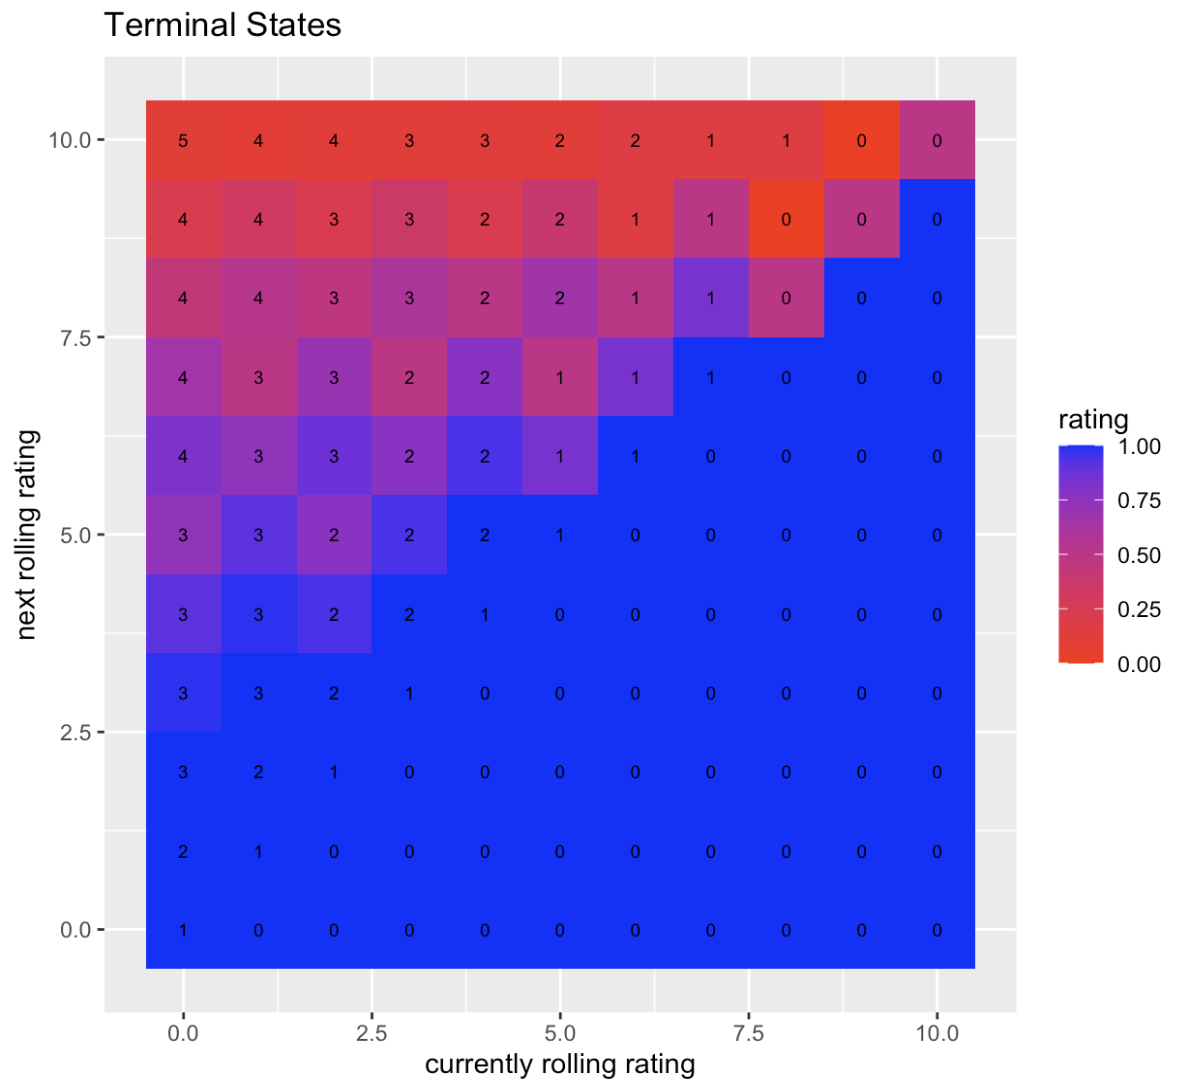
\includegraphics[width=6.5cm]{Screenshot 2023-12-12 at 20.21.12.png}
%     \caption{Terminal States}
%     \label{fig:2figsA}
%     }
%     \qquad
%     \begin{minipage}{6cm}
%     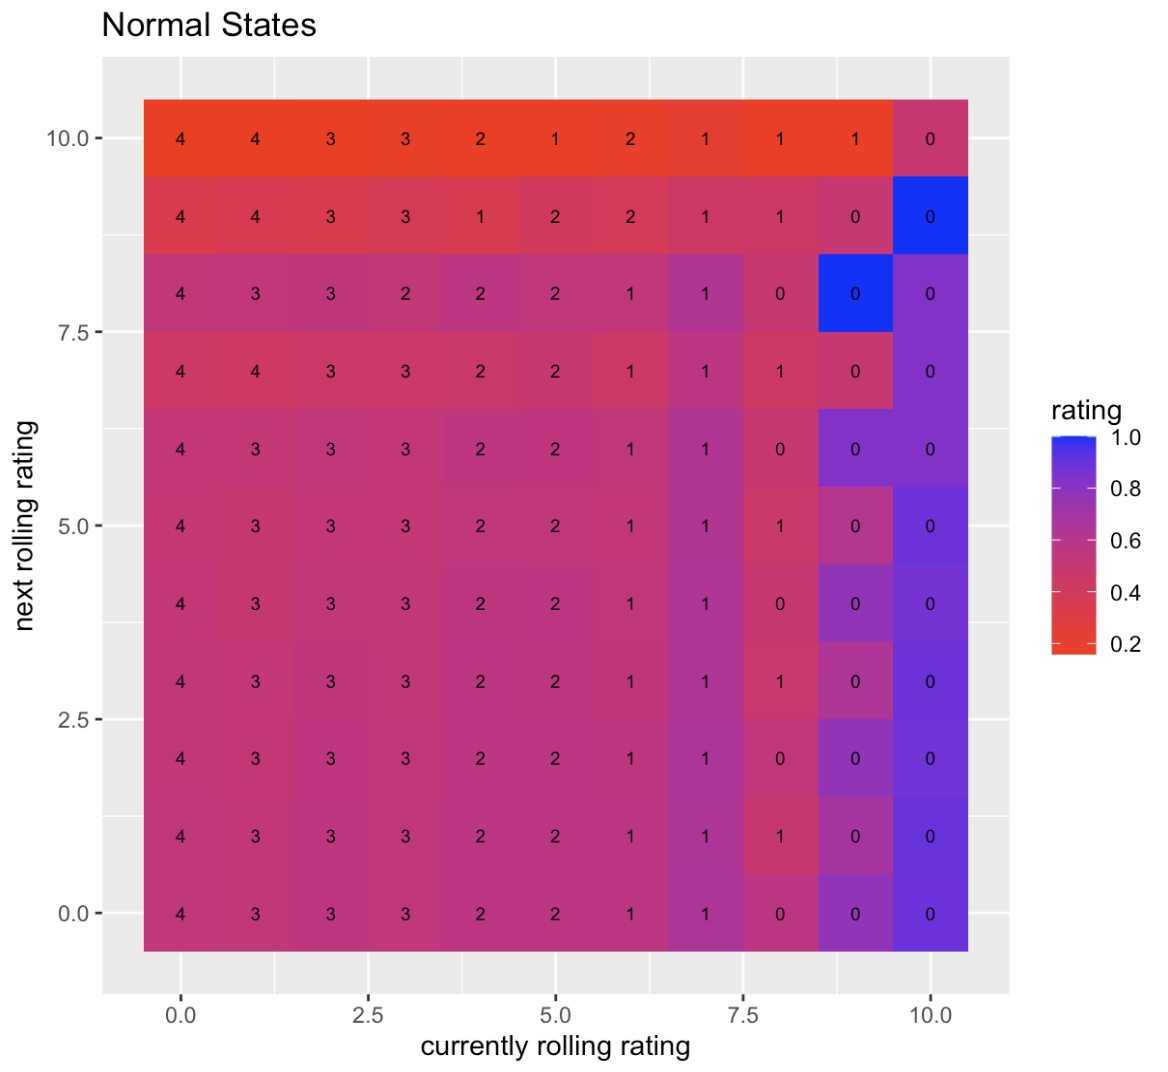
\includegraphics[width=6.5cm]{Screenshot 2023-12-12 at 20.22.15.png}
%     \caption{Normal States}
%     \label{fig:2figsB}
%     \end{minipage}
%     \end{figure}

%% ----- SECTION: INTRODUCTION TO GREED ----- %%

\section{Introduction to Greed}

%% ----- SUBSECTION: WHAT IS GREED ----- %%

\subsection{What is Greed?}

Greed is a two-player, probabilistic, game that could be described as ``kinda like blackjack with dice''. Each player starts with a score of 0, which we'll label player score $s_p = 0$ and opponent score $s_o = 0$. The game also has some max score $M$ and, of course, each dice has $s$ sides. One player will start. They may choose any natural number $n \in \mathbb{N}^0$ (including zero) of dice to roll. Once they roll, they will then add the sum of all the dice together and add that to their score. Then the opponent will choose to roll some $n$ number of dice and repeat, until one of two terminal states is reached.

In the first option, a player's score goes over $M$, i.e. and they go bust. In this case, they lose, so we'll say that their rating -- the heuristic measure that we use to measure how good a position is -- is 0, and thus their opponents rating is 1. 

In the second option, a player can choose to roll 0 dice. This will initiate the last turn. The other player will then have one more chance to roll. The winner is the player who has the higher score that is not over $M$. In the case of a tie, rating is 1/2 for each player. 

So for now, rating is defined
%
$$
\text{rating} = \begin{cases}
	1 & \text{if win} \\
	\frac{1}{2} & \text{if tie} \\
	1 & \text{if lose} 
\end{cases}
$$
%
For clarity, all examples will use a game environment where $M = 10$ and $s = 3$, but our analysis will extend to any $s \in \mathbb{N}, M \in \mathbb{N}$. And notably, the classic game of greed has $M = 100$, $s = 6$.

%% ----- SUBSECTION: WHY ----- %%

\subsection{Why}

At this point, you may be asking why investigate optimal play in a completely unknown game that was most likely made up my Reed CS faculty? 

I could explain that the optimization of probabilistic processes has relevance across various applications and industries, including finance, operations research, and engineering. Decision-making in uncertain environments is a common challenge, and optimizing strategies based on probabilistic models can lead to more informed and effective outcomes.

But come on. You didn't come to this paper to hear about the applications of game thoery, and I didn't write this paper to talk about it. I wrote this paper because 

\begin{enumerate}
\item I really like this problem. The idea of optimizing games is a exciting and challenging problem, and greed is just the kind of bit-sized game that allows for interesting problem-solving without becoming a behemoth (though I'd argue that it kinda is. The amount of rabbit holes that I've went down for this mini-thesis is insane.) and

\item My original algorithm lost to a basic if-else chain, and I'm filled with overwhelming spite. So much spite that I've spent the last 2 years thinking about it, only to spend \textit{this much} time optimizing it (given heuristic of rating / how states relate to each other - we'll get to it) 
\end{enumerate}

%% ----- SUBSECTION: METHEMATICAL FRAMEWORK ----- %%

\section{Mathematical Framework}

Before beginning any calculations, it is necessary to first setup the problem space and how it will be conceptualized mathematically. By the nature of it's structure -- its a markov process -- Greed is well-split into two kinds of states; terminal states, which denote the last turn of the game, and normal turns, representing all other states. 

Both normal and terminal states can be thought of as 2 by 2 boards with dimensions $M+1$ by $M+1$, representing all possible states for player and opponent. Notably, the x-axis designates the player presently up to roll, while the y-axis designates the player who has just rolled. So a state of $(5, 8)$ could mean you have $5$, and the opponent has $8$, or vise versa, depending on whose turn it is. This might seem like a unintuitive framework, but it well-suits this game becuase of how it alternates back and forth between players. Thus it avoids redundancy, because as we'll see later, rating is complementary.

Therefore, any state $S$ can be defined by the tuple $(s_0, s_1, l)$, where $s_0$ denotes the score of the player currently rolling, $s_1$ is the score of the other player, and $l$ is an indicator variable for whether the current turn is a terminal turn or normal turn.

For an example of how this all fits together, consider a scenario where the state is $(5, 8, 0)$, with your turn to roll. You roll 2 dice, and get a sum of 4. So the state is now $(8, 9, 0)$. Notice that the eight has gone from the second argument to the first. This is because it's the opponent's turn, so their score is listed as being "up to roll". 

So in general, in some normal state $(s_0, s_1, 0)$, rolling $n > 0$ dice with sum $t$ makes the next state $(s_1, s_0 + t, 0)$, and in the case $n = 0$, the next state is $(s_1, s_0, 1)$. In some terminal state $(s_0, s_1, 1)$, rolling getting some sum $t$ will make the next state $(s_0, s_1 + t, 1)$, concluding the game.

%% ----- SECTION: PMF OF N INDEPENDENT AND IDENTIALLY DISTRIBUTED DISCRETE UNIFORM RANDOM VARAIBLES WITH S OUTCOMES ----- %%

\section{PMF}

Before beginning anything about actually deriving, it is imperative that we first find the most essential tool for solving this problem. What is the probabiltiy mass function of the sum of $n$ independent and identically distributed dice? 

% So knowing the procedure to find the optimal $n$ and $\text{rating}$, this paper reaches the elephant in the room, which underpins every decision in the game. What is the pmf of the sum of $n$ independent and identically distributed dice? Ex

First, consider just a single dice. It has pmf
%
$$
D_{i}^{(s)}(d) = \begin{cases}
    \frac{1}{s} & \text{if } d \in \{1, \ldots, s \} \\
    0 & \text{otherwise}
\end{cases}
$$
%
So let the random variable $T$ denote the sum of $n$ iid random dice, each with $s$. It can thusly be written
%
$$ 
T: \left(\mathbb{N}^{0}\right)^n \to \mathbb{R}, T \coloneqq D_{1}^{(s)}(d_1) + \cdots + D_{n}^{(s)}(d_n) 
$$
%
Therefore, our goal is to find the pmf of $T$, which is notated $\textbf{p}_{T}^{(n, s)}(t)$, dependent on parameters $n, s$. 

There are multiple ways to go about finding this pmf. One such method involves combinatorics. This paper will instead use moment-generating functions and polynomials.

%% --- multinomail lemma --- %%

\begin{lemma}
    Let $M_{T}^{(n, s)}$ be the moment generating function of $T$, then 
    $$ M_{T}^{(n, s)} = \frac{1}{n^s} (e^{t} + e^{2t} + \cdots  + e^{st})^n $$
\end{lemma}

%% --- proof of multinomail lemma --- %%

\begin{proof}
    Recall the pmf of $D_{i}^{(s)}$. It's moment generating function is defined as
    %
    $$
    M_{D_{i}^{(s)}}(t) = \mathbb{E}[e^{tD_{i}^{(s)}}] = \frac{1}{s}(e^{t} + e^{2t} + \cdots + e^{st})
    $$
    %
    Since $D_{i}^{(s)}$ are all independent and identically distributed,
    %
    \begin{align*}
        M_{T}(t) &= \mathbb{E}[e^{tT}] = \mathbb{E}[e^{t(D_{1}^{(s)} + \cdots + D_{n}^{(s)})}] = \prod_{i = 1}^{n} \mathbb{E}[e^{tD_{i}^{(s)}}] \\
        &= \prod_{i = 1}^{n} \left[\frac{1}{s}(e^{t} + e^{2t} + \cdots + e^{st}) \right] \\
        &= \frac{1}{s^n} (e^{t} + e^{2t} + \cdots + e^{st})^n
    \end{align*}
\end{proof}

Probability distributions and moment generating functions have a one-to-one correspondance. So for a discrete random variable $X$ with probability distribution
%
$$ 
f(x_i) = P(X = x_i) = p_i \text{ for } i = 1, 2, \ldots k 
$$
%
then it's mfg is
%
\begin{align*}
    M_X(t) &= \mathbb{E}[e^{tX}] = \sum_{x} e^{tx} \cdot f(x) =  \\ 
    &= p_1 \cdot e^{tx_1} + p_2 \cdot e^{tx_2} + \cdots + p_k \cdot e^{tx_k}.
\end{align*}
%
and visa verse (like in [\textit{HW 6, 2.1}]).

It follows that for $t = 1$, the coefficients of the moment generating function are the probabilities of the random variable. Specifically, $P(X = x)$ is the coefficient of the term $e^x$. Extending this principle to $T$, the coefficients of the multinomial outlines in \textbf{Lemma 1} correspond to the probabilities of rolling that corresponding sum, so $P(T = x)$ is still the coefficient of the term $e^x$.

For clarity, let's use the interchangable but more intertpretable multinomial $\frac{1}{s_n}(x + x^2 + \cdots + x^s)^n$. The coefficients of $g(x)$ are the same as the coefficients of $M_T$, so the math is the same.

%% --- closed formula lemma --- %%

\begin{lemma}
    For a multinomial $g(x) = \frac{1}{s_n}(x + x^2 + \cdots + x^s)^n$, the coefficient of the $k$\textsuperscript{th} term $x^k$ is given by
    $$ \frac{1}{s^n} \sum_{l = 0}^{\lfloor\frac{t-n}{s} \rfloor} (-1)^k \binom{n}{k} \binom{k-sk-1}{n-1} $$
\end{lemma}

%% --- proof of closed formula lemma --- %%

\begin{proof}
    Using the geometric series, rewrite
    %
    $$
    g(x) = \frac{1}{s_n}(x + x^2 + \cdots + x^s)^n = \frac{1}{s_n} \left(\frac{x(x^s-1)}{x-1} \right)^n = \frac{1}{s_n} \frac{x^n(x^s-1)^n}{(x-1)^n}
    $$

    Looking at the numerator $(x^s - 1)^n$, we can expand this with the binomial theorem, \textit{Fact D.2. [ASV]}
    %
    $$
    (x^s+1)^n = \sum_{i = 0}^{n} \binom{n}{i} (x^s)^i \cdot (-1)^{n-i}
    $$
    %
    multiplying by $x^n$, this becomes
    %
    $$
    x^n(x^s+1)^n = \sum_{i = 0}^{n} \binom{n}{i} x^{si+n} \cdot (-1)^{n-i}
    $$ 

    Looking at the denominator $(x-1)^{-n}$. Rewrite this to $(-1)^{-n} \cdot (1-x)^{-n}$. Again this can be rewritten as the sum of binomial cofficients, but this time $(1-x)^{-n}$ is a binomial series (an expansion of the binomial theorem for complex exponents), in specific the negative binomial. Starting by expanding the taylor series,
    %
    \begin{align*}
        f(x) = (1-x)^{-n} &= \sum_{j = 0}^{\infty} \frac{f^{(k)}(0)}{j!} x^j \\
        &=1 + nx + \frac{n(n+1)}{2!} x^2 + \frac{n(n+1)(n+2)}{3!} x^3 + \cdots \\
    \end{align*}  
    %
    and since 
    %
    $$
    \frac{n(n+1)(n+2) \cdots (n+j-1)}{j!} = \binom{n+j-1}{j}
    $$
    %
    that means
    %
    \begin{align*}
        1 + nx + \frac{n(n+1)}{2!} x^2 + \frac{n(n+1)(n+2)}{3!} x^3 + \cdots = \sum_{j = 0}^{\infty}\binom{n+j-1}{j} x^j
    \end{align*}
    %
    and thus the denominator is 
    %
    $$ 
    (-1)^{-n} (x-1)^{-n} = (-1)^{-n} \cdot\sum_{j = 0}^{\infty}\binom{n+j-1}{j} x^j 
    $$

    So together, the full equation of $g(x)$ becomes the product of the numerator and denominator as such  
    %
    $$
    g(x) = \left(\sum_{i = 0}^{n} \binom{n}{i} x^{si+n} \cdot (-1)^{n-i} \right) \left((-1)^n \cdot \sum_{j = 0}^{\infty}\binom{n+j-1}{j} x^j \right)
    $$ 
    %
    Moving the $(-1)^{-n}$ to the other equation and then simplifying $(-1)^{-i}$ to $(-1)^i$  
    %
    $$
    g(x) = \left(\sum_{i = 0}^{n} (-1)^i \binom{n}{i} x^{si+n} \right) \left(\sum_{j = 0}^{\infty}\binom{n+j-1}{j} x^j \right)
    $$ 
    %
    The finite sum can be though of as a infinite sum that takes 0 whenever $i > n$. This allows us to use Cauchy product to get the coefficients, which generally states that:
    %
    $$
    \left(\sum_{i=0}^{\infty} a_i x^i \right) \left(\sum_{j=0}^{\infty} b_j x^j \right) = \sum_{k=0}^{\infty} c_k x^k
    $$  
    %
    Where the coefficients $c_k$ are defined as
    %
    $$
    c_k = \sum_{l = 0}^{k} a_l b_{k-l}
    $$

    Doing some careful accounting of coefficients (\textit{authors note:} I genuinely don't know what happened for this step), this yields the double summation and result
    %
    $$
    g(x) = \frac{1}{s^n} \sum_{k = 0}^{\infty} \left(\sum_{l = 0}^{\lfloor\frac{k-n}{s} \rfloor} (-1)^k \binom{n}{k} \binom{k-sl-1}{n-1} \right) x^k
    $$
    %
    Which means that the coefficient of $x^k$ is 
    %
    $$
    \frac{1}{s^n} \sum_{l = 0}^{\lfloor\frac{t-n}{s} \rfloor} (-1)^k \binom{n}{k} \binom{k-sk-1}{n-1}
    $$ 
\end{proof}

%% --- big pmf theorem --- %%

By recognizing that the coefficients of the multinomial directly represent the probabilities in the probability mass function (pmf), as previously explained, we can straightforwardly apply \textbf{lemma 2} to determine the pmf of $T$ is given by.
%
\begin{theorem}{probability mass function of $T^{(n, s)}$}
    $$
    \textbf{p}_{T}^{(n, s)}(t) = \frac{1}{s^n} \sum_{k = 0}^{\lfloor\frac{t-n}{s} \rfloor} (-1)^k \binom{n}{k} \binom{t - s \cdot k - 1}{n-1}
    $$
\end{theorem}

With proof as just completed.

%% ----- SECTION: OPTIMIZATION OF TERMINAL STATES ----- %%

\section{Optimization of Terminal States}

\begin{figure}[h]
    \centering
    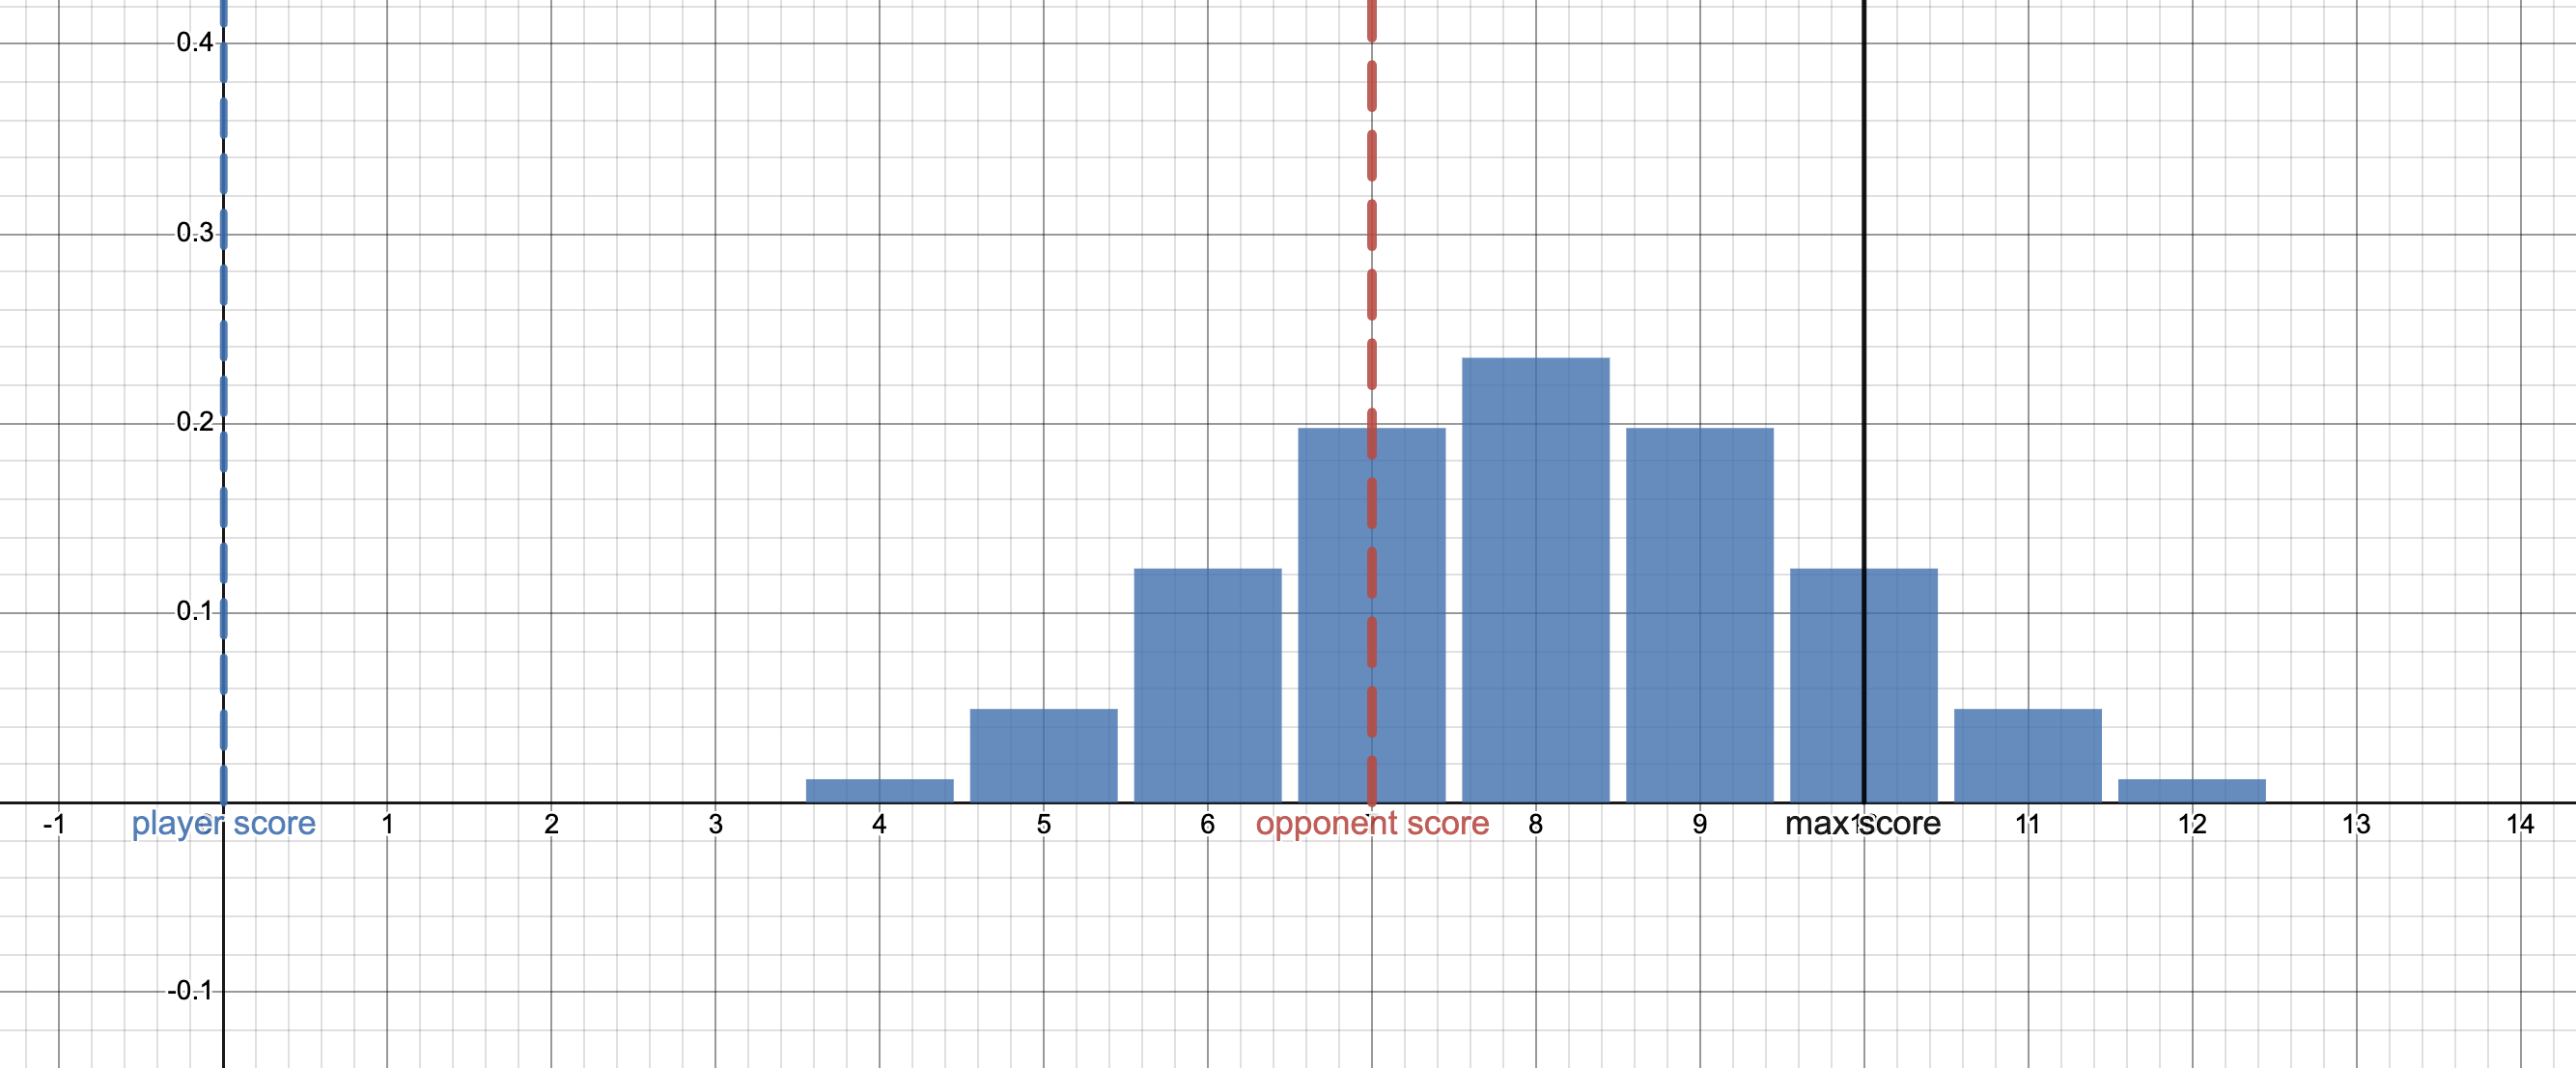
\includegraphics[width=0.9\textwidth]{Screenshot 2023-12-09 at 21.07.12.png}
    \caption{Visual Demonstration of Terminal States}
\end{figure}

Considering that normal states will eventually terminate at terminal states, it is natural to first consider and calculate these states.

In order to find the optimal action in terminal states, it is useful to reframe the problem as ``What is the optimal $n$ to maximize the probability of getting a new score $s_p + t$ between $s_o$, and $M$?" Or more precisely, given a state $(s_p, s_o, 1)$, what is the optimal $n$ such that the expected rating is maximized. With rating being the heuristic that we defined to determine the optimal actions -- and to give a measure of the probability of winning that also includes ties. 
%
\begin{equation}
    \text{rating}((s_p, s_o, 1), n) \coloneqq \sum_{t = s_o+1}^{\text{M}} \textbf{p}_{T}^{(n, s)}(t - s_p) + \frac{1}{2} \cdot \textbf{p}_{T}^{(n, s)}(s_o - s_p)
\end{equation}
%
where the summation describes the weighted sum of all next states given $n$, weighted according to their probability (transition matrix), hence rating is the expectation of its next possible states. 

Since $n_{\star}$ is the optimizer of rating, it is given by
%
\begin{equation}
    n_{\star}(s_0, s_1, 1) \coloneqq \text{argmax}_n \left\{ \text{rating}((s_0, s_1, 1), n) \right\}
\end{equation}
%
Notice that the optimal rating comes for free. It's the rating that was optimized for in finding $n_{\star}$, so no additional work is required.
%
\begin{equation}
    \text{rating}_{\star}((s_p, s_o, 1), n_{\star}) \coloneqq \text{rating}((s_p, s_o, 1), n_{\star})
\end{equation}

%% ----- SECTION: CALCULATING TERMINAL STATES ----- %%

\section{Calculating Terminal States}

However, for practical computational purposes, it is crucial to determine a systematic and efficient approach. This would avoid the need to evaluate every possible $n$ from $s_o - s_p$ up to $M - s_p$, which is wildly impractical at larger board sizes. When should the algorithm stop?

There are in fact certain states where the choice is immediately obvious without any need for calculations with pmfs. Thsese states can be broken into 2 types that I'll call \textit{forfeit} and \textit{certain victory}. 

In \textit{forfeit} states, the opponent decided to end the game while they were behind, which guarantees that you win by doing nothing and rolling 0 dice. This state will never occur in optimal Greed because a player that is behind would never roll 0 dice, since their rating would be 0, and they can always improve by rolling some optimum $n$ dice. 

In \textit{certain victory} states, the relation between the player $s_p$ and oppoent $s_o$ compared to the opponent and the maximum $M$ is such that for some $n$, all possible resulting sums $s_p + t$ are in the range $s_o < s_p + t  \leq M$. Thus there is some $n_{\star}$ with a 100\% win rate.

However, these states are edge cases in optimal greed. For the most part, all terminal states that are reached will not have a move which assured victory. These are the states where an optimization algorithm is needed.

In order to find that algorithm, first let's gain some insight into some of the properties of this distribution.
%
\begin{lemma}{Expectation of $\textbf{p}_{T}^{(n, s)}$}
    $$ \mathbb{E}[T^{(s, n)}] = \frac{n(s+1)}{2} $$
\end{lemma}
%
\begin{proof}
    \begin{align*}
        \mathbb{E}[T^{(s, n)}] &= \mathbb{E}[D_{1}^{(s)} + \cdots + D_{n}^{(s)}] = \mathbb{E}[D_{1}^{(s)}] + \cdots + \mathbb{E}[D_{n}^{(s)}] \\
        &= n \cdot \mathbb{E}[D_{1}^{(s)}] = n \cdot \sum_{k=1}^{s} k \cdot \frac{1}{s} = n \cdot \frac{1}{s} \cdot \frac{(s)(s+1)}{2} \\
        &= \frac{n(s+1)}{2} \\
    \end{align*}
\end{proof}

\begin{lemma}{Variance of $\textbf{p}_{T}^{(n, s)}$}
    $$ \text{Var}[T^{(n, s)}] = \frac{s^2 - 1}{12}  $$
\end{lemma}
%
\begin{proof}
    \begin{align*}
        \text{Var}[T^{(n, s)}] &= \text{Var}[D_{1}^{(s)} + \cdots + D_{n}^{(s)}] = \text{Var}[D_{1}^{(s)}] + \cdots + \text{Var}[D_{n}^{(s)}] \\
        &= n \cdot \text{Var}[D_{1}^{(s)}] 
    \end{align*}
    %
    The variance of $D_{1}^{(s)}$ is given by $\mathbb{E}\left[(D_{1}^{(s)})^2 \right] - \mathbb{E}\left[D_{1}^{(s)} \right]^2$ as stated in \textit{Fact 3.48 [ASV]}.
    %
    \begin{align*}
        \mathbb{E}\left[\left(D_{1}^{(s)}\right)^2 \right] &= \sum_{k=1}^{s} k^2 \cdot \frac{1}{s} = \frac{1}{s} \frac{s(s+1)(2s+1)}{6} = \frac{(s+1)(2s+1)}{6} \\
        \mathbb{E}[T^{(n, s)}] &= \sum_{k=1}^{s} k \cdot \frac{1}{s} = \frac{1}{s} \cdot \frac{(s)(s+1)}{2} = \frac{s+1}{2}
    \end{align*}
    %
    Thus the expectation of a single die $D_{1}^{(s)}$ is given by 
    %
    \begin{align*}
    \text{Var}[D_{1}^{(s)}] &= \mathbb{E}\left[(D_{1}^{(s)})^2 \right] - \mathbb{E}\left[D_{1}^{(s)} \right]^2 \\
    &= \frac{(s+1)(2s+1)}{6} - \left(\frac{s+1}{2} \right)^2 \\
    &= \frac{2s^2 + 3s + 1}{6} - \frac{s^2 + 2s + 1}{4} \\
    &= \frac{4s^2 + 6s + 2}{12} - \frac{3s^2 + 6s + 3}{12} \\
    &= \frac{s^2 - 1}{12}
    \end{align*}
    %
    Thus the variance of $T$ is
    %
    $$
    \text{Var}[T^{(s, n)}] = n \cdot \text{Var}[D_{1}^{(s)}]  = n \left(\frac{s^2 - 1}{12} \right)
    $$
\end{proof}

%% --- conjecture begins --- %%

\begin{figure}[h]
\centering
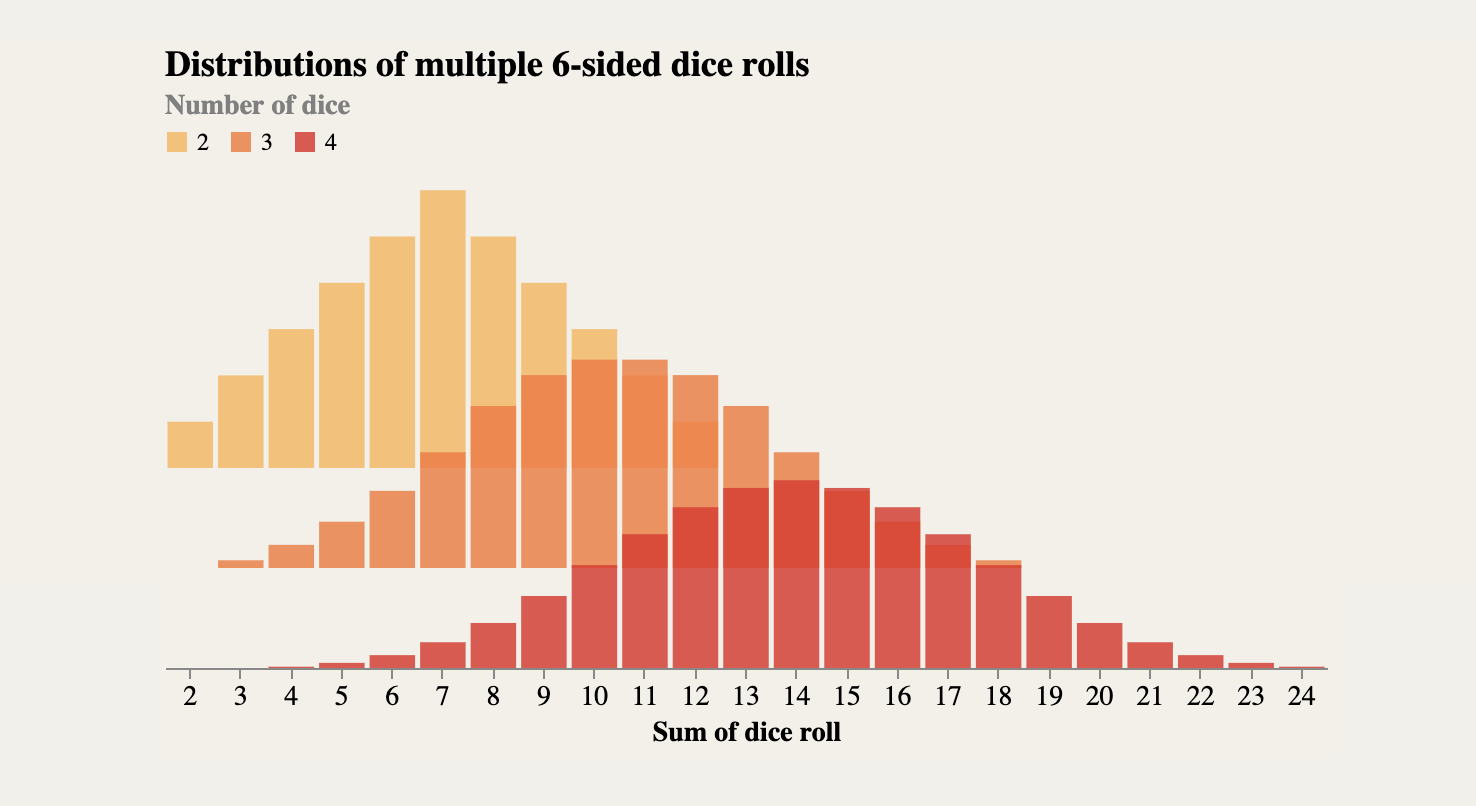
\includegraphics[width=0.8\textwidth]{Screenshot 2023-12-10 at 19.58.36.png}
\caption{Distributions of $n = 2, 3, 4$ with $s = 6$}
\end{figure}

To derive an algorithm however, this paper will make a few significant conjectures:
%
\begin{conjecture}
    For any $n$ with corresponing $T^{(n, s)}$ with mean $s_p + \mathbb{E}[T^{(n, s)}]$ above $\frac{s_o + M}{2}$, rating is monotonically decreasing as a function of $n$.
\end{conjecture}
%
\begin{conjecture}
    Rating as a function of $T^{(n, s)}$ with parameter $n$ is unimodal.
\end{conjecture}
%
(\textit{authors note:} I settled on these higher level conjectures for brevity)

With this, deriving algorithm is simple. 

\begin{enumerate}
\item Find the smallest $n$ such that $s_p + \mathbb{E}[T^{(n, s)}] > \frac{s_o + M}{2}$ 
%
\begin{align*}
    & s_p + \mathbb{E}[T^{(n, s)}] > \frac{s_o + M}{2} \implies s_p + \frac{n(s+1)}{2} > \frac{s_o + M}{2} && \text{from lemma 3} \\
    \implies &  \frac{n(s+1)}{2} > \frac{s_o + M - 2 s_p}{2} \implies n > \frac{M + s_o - 2 s_p}{s+1}
\end{align*}

\item Calculate rating, keeping track of the highest one. When the rating starts to decrease, stop, and select the greatest $\text{rating}_{\star}$ and corresponding $n_{\star}$
\end{enumerate}

This will work because the rating distribution is unimodal, i.e. \textbf{conjecture 2}. From \textbf{conjecture 1}, starting above $n_0 = \frac{M + s_o - 2 s_p}{s+1}$ means all $n > n_0$ have decreasing rating. This implies that $n_0$ must be to the left of the mean of the rating distribution. That means that when rating begins to decrease, we've transitioned from above the mean to below the mean. And since rating is unimodal, this must be the true maxima. \newline

%% --- visualizing optimal n and ratings --- %%

Applying the algorithm to the game with $M = 20, s = 3$, the terminal states are visualized below, with the label corresponding to the $n_{\star}$ and the color corresponding to the rating.

\begin{figure}[h]
    \centering
    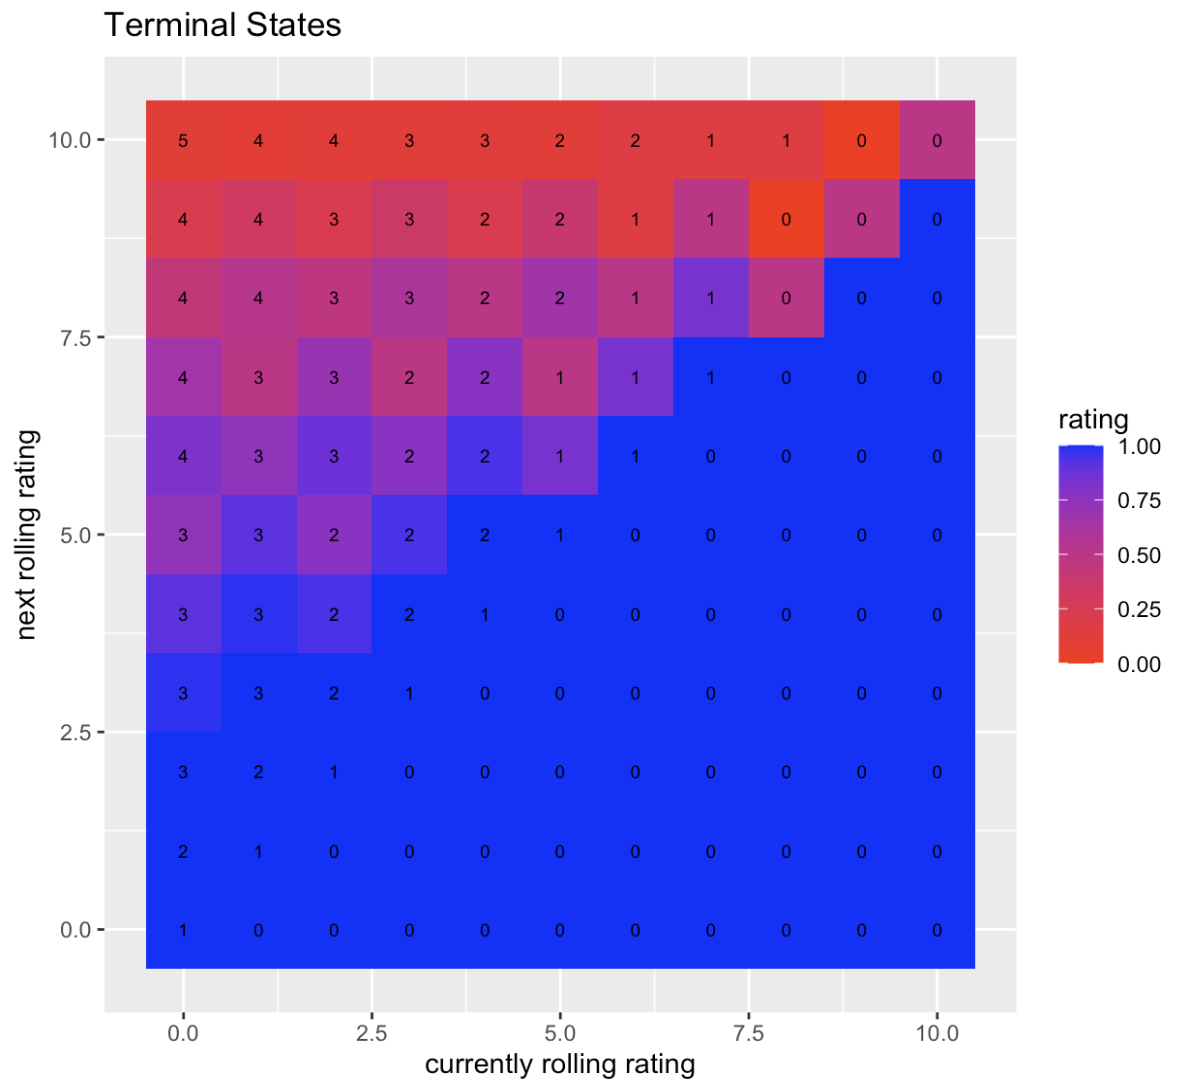
\includegraphics[width=0.7\textwidth]{Screenshot 2023-12-12 at 20.21.12.png}
    \caption{Optimal Actions and Ratings for Terminal States}
\end{figure}

%% ----- SECTION: OPTIMIZATION OF NORML STATES ----- %%

\section{Optimization of Normal States}

Finally, we can shift focus to normal states. Normal states are differentiable from terminal states because the player has to not only consider their current state but which states they could move to next, and how favorable those states are. 

The goal for this section is twofold: generate some function which can determine the rating of a given state, and derive an algorithm which can implement that function. 

The optimal rating is defined in the same way as it is for terminal states: The expectation of the rating for the next possible states $S_1$ given some $n$. Or in other words, the weighted sum of the rating over all possible next states $S_1$, weighted by the transition matrix between the current and next states for $n$. 

Let's give an example. Imagine that the optimal $n_{\star}$ and $\text{rating}_{\star}$ for every other state is known. 

Consider rolling $2$ dice at state $(2, 6)$. You could end up at any of the following states: $S_1 = \{(6, 4), (6,5), (6,6), (6,7)\}$. So since we know the rating of all these states, we can calculate the rating given $n$ by taking the weighted sum over $S_1$, with weights given by the pmf of $T$, i.e. $\textbf{p}_{T}^{(n, s)}(2), \ldots, \textbf{p}_{T}^{(n, s)}(4)$.

It's important to note that the rating at a resulting state like $(6, 4)$ represents the opponent's rating. However, rating is complementary, as demonstrated
%
\begin{align*}
s_o &= \sum_{t = s_o+1}^{\text{M}} \textbf{p}_{T}^{(n, s)}(t - s_p) + \frac{1}{2} \cdot \textbf{p}_{T}^{(n, s)}(s_o - s_p) \\
&= 1 - \left(\sum_{t = 0}^{s_o - 1} \textbf{p}_{T}^{(n, s)}(t - s_p) + \sum_{t = M}^{\infty} \textbf{p}_{T}^{(n, s)}(t - s_p)  + \frac{1}{2} \cdot \textbf{p}_{T}^{(n, s)}(s_o - s_p)\right) = s_p
\end{align*}

Hence, the rating for landing on a state $S$ is $1-\text{rating}(S, n_{\star})$, where $n_{\star}$ is the optimal $n$ for that state. 

So the rating function is given by
%
\begin{equation}
    \text{rating}((s_p, s_o, 0), n) \coloneqq \begin{cases}
        \sum_{t = n}^{s \cdot n} 1 - \text{rating}((s_o, s_p + t, 0), n_{\star}) & \text{if } n > 0 \\
        1- \text{rating}((s_o, s_p, 1), n_{\star}) & \text{if } n = 0
    \end{cases}
\end{equation}
%
Thus the optimal $n_{\star}$ given any possible state $S$, normal or terminal is now defined to be
%
$$
n_{\star} = \text{argmax}_{n} \left\{\sum_{t = n}^{s \cdot n} 1 - \text{rating}((s_o, s_p + t, \{0 \text{ if } n = 1 \text{ else } 0\}) \right\}
$$
%
with the rating function being either equation (1) or (4) depending on whether its a terminal state or normal state.

With $\text{rating}_{\star}$ defined the same as equation (3).

Remark: rating is guaranteed to produce a $n_{\star}$ and $\text{rating}_{\star}$ since eventually the state wil either be terminal (which has concrete $n_{\star}$ and $\text{rating}_{\star}$) or go bust.

%% ----- SECTION: CALCULATING NORMAL STATES  ----- %%

\section{Calculating Normal States}

While the recursive approach with momoization, (the classic dynamic programming solution) would suffice as an algorithm to determine normal states, this either does a massive amount of duplicate work, or adds significant complexity. Instead, this paper suggests an iterative approach that utilizes a optimal ordering of calculating states.  

Consider that we've already calculated optimal actions and ratings for terminal states. This means that the only unknowns are other normal states. 

So what if we looked at the state $(M, M, 0)$? In this state, the only possible move would be either rolling $0$ and going to a terminal state, or going bust. Looking at the states adjacent to $(M, M, 0)$, these states can also go to a terminal state or go bust. They could also transition to $(M, M, 0)$, but that state is already calculated, so it still works. 

In fact, because scores only increase, as the game goes on the sum of $s_p + s_o$ will always increase. So if we calculate the states from the maximum possible sum $s_p + s_o$ and decrease, then we should never reach a state that we don't already know the answer to. This is the optimal ordering.

% \begin{figure}[h]
%     \centering
%     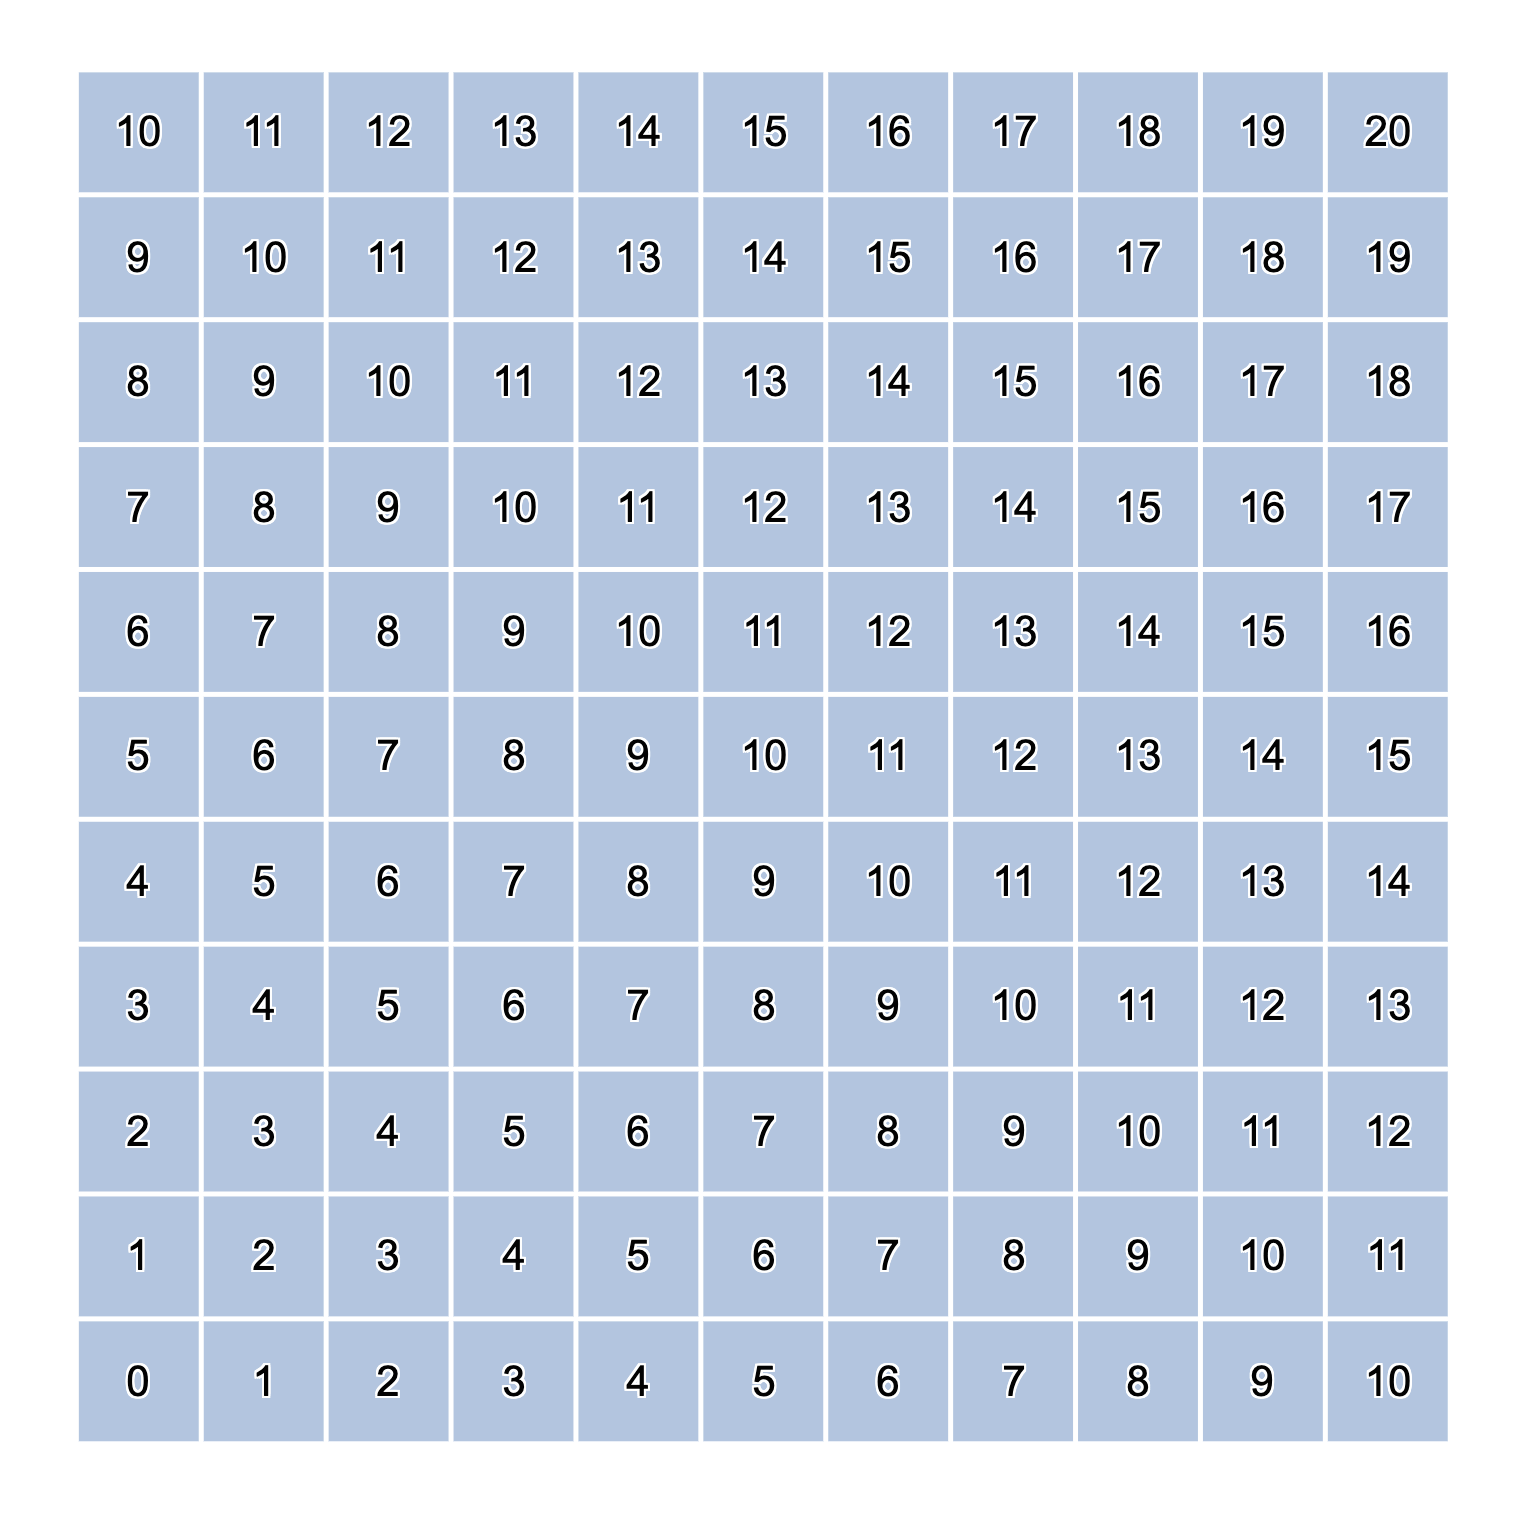
\includegraphics[width=0.5\textwidth]{Screenshot 2023-12-10 at 01.11.06.png}
%     \caption{Show Ordering of Calculating Optimal Actions}
% \end{figure}

Along with the ordering, its also important to find a cutoff for checking $n$ values, like in terminal states. Since it's hard to know how normal states will effect each other, the upper bound will have to be less tight than it is for terminal states. 

We can make this upper bound $n_0$ be where the mean $s_p + \mathbb{E}[T^{(n, s)}]$ is greater than $M$, calculated to be
%
$$
s_p + \mathbb{E}[T^{(n, s)}] > M \implies s_p + \frac{n(s+1)}{2} > M \implies n > \frac{2(M - s_p)}{s+1}
$$
%
This works since any $n > n_0$ will have the exact same next states but every probability will be smaller than it would be for $n_0$. \newline

%% --- visualizing optimal n and ratings --- %%

Applying the algorithm to the game with $M = 20, s = 3$, the normal states are visualized below, with the label corresponding to the $n_{\star}$ and the color corresponding to the rating.

\begin{figure}[h]
    \centering
    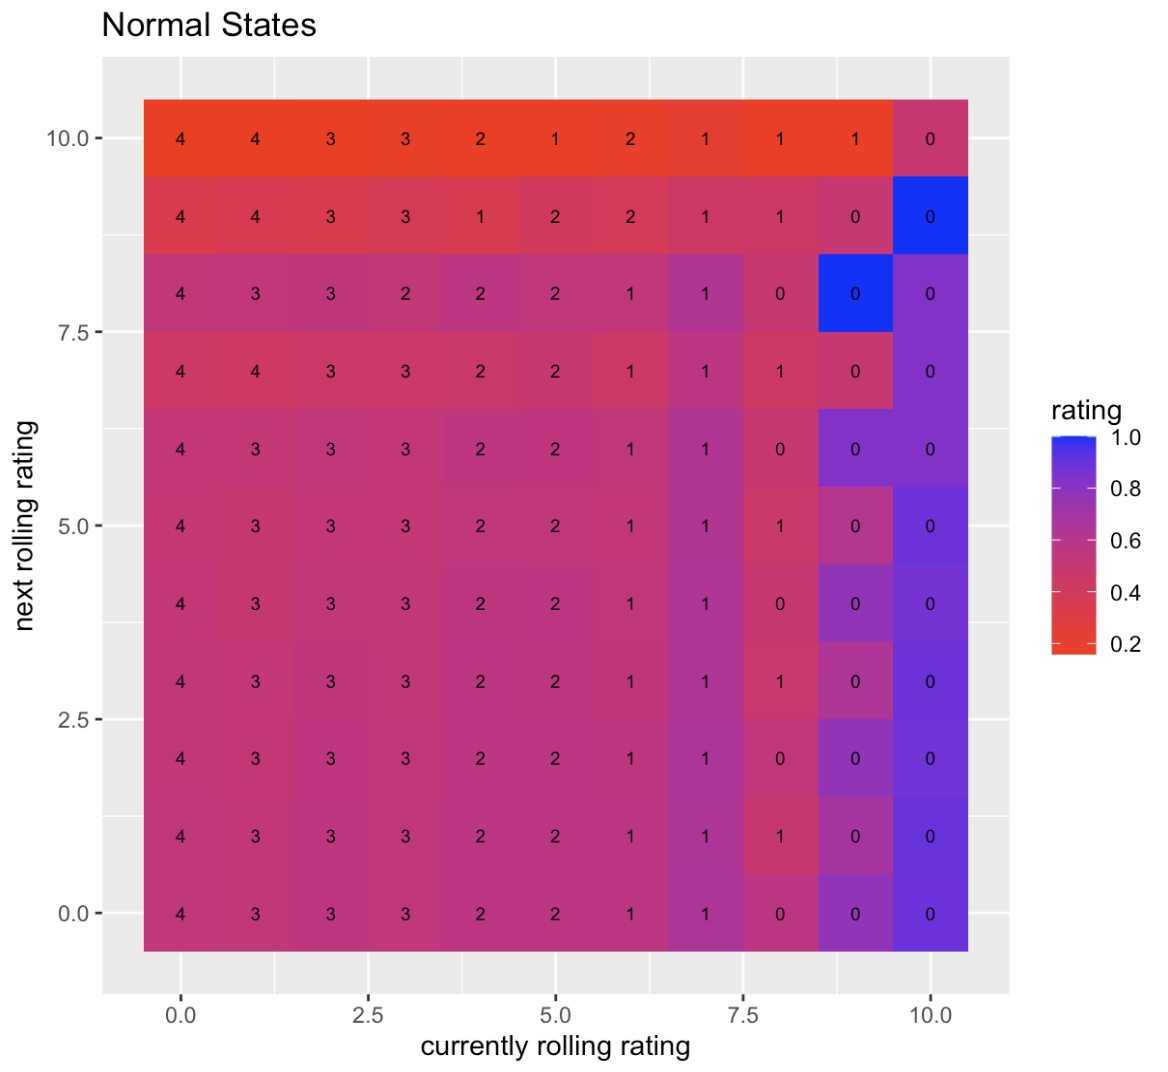
\includegraphics[width=0.7\textwidth]{Screenshot 2023-12-12 at 20.22.15.png}
    \caption{Optimal Actions and Ratings for Normal States}
\end{figure}

%% ----- SECTION: CONCLUSION ----- %%

\section{Conclusion}

%% --- general findings --- %%

With both normal and terminal states calculated, we have thusly achieved our stated aim of finding some optimal strategy for playing greed. In terms of markov chains, we've tuned the paramter $n$ in order to optimize a transition matrix over the game states which optimizes for a heuristic that we defined called rating. 

%% --- important results --- %%

In doing so, we've defined a few significant functions. Primarily, we've defined a function for determining the rating of any possible state $S$, and from that also defining an optimal $n$ and rating, denoted $n_{\star}$ and $\text{rating}_{\star}$. In order to do so, w also derived the pmf for the sum of $n$ fair, independent and identially distribed dice. 

%% --- limitations --- %%

As stated previously, there are a few limitations to this analysis. the biggest, of course, is that rating is not an objective function of success. A player could determine that tying is just as bad as winning, and have a unique, yet completely valid rating metric. Additionally, it is unclear whether defining rating as the weighted sum of the resulting states $S_1$ is truly the optimal way to relate ratings to each other. 

%% --- additional research --- %%

As for additinal research, there are many possible routes through which further research could proceed. Of primary relevance is a more mathematically rigourous framework. This paper breifly touches on many important and relevant ideas: markov decision chains, mathemical optimization for dynamic programming, reinforcement learning, etc. This problem has significant overlap with all of these fields. A more thorough analysis of this problem which incorporates these concepts would be a welcome addition.

Additionally, there are many open questions that further research could study. Top among them is to determine whether the conjectures described in ``Calculating Terminal State'' are in fact true, and thus whether the algorith is sound. Another potential path is to investigate normal states, and see if there is some pattern which can help improve the upper bound. 

As Greed is completely unexplored, there is massive room for further discovery and investigation in optimization, patterns, and more.

%% --- additional --- %%

One additional note: A corollary of finding the optimal rating for every state is that we can determine whether going first has a benefit for rating, and how much. It turns out that for a game environment of $M = 10, s = 3$, going first has a rating of $0.54$, so it is very slightly adventagous to go first. And the rating implies that going first improves the chance of winning vs losing by about 4\%. Take that conjecture as you will.

%% --- code appendic --- %%

All code used to calculate the results is available here: https://github.com/Approximately-Equal/Greed.git

%% ----- BIBLIOGRAPHY / REFERENCES ----- %%

\begin{thebibliography}{3}

\bibitem{Introduction to Probability [ASV]}
Introduction to Probability [ASV],
\\\texttt{Anderson, D. F., Seppäläinen, T., \& Valkó, B. (2018). Introduction to probability. Cambridge: Cambridge University Press.}


\bibitem{The probability distribution of the sum of several dice: Slot applications}
The probability distribution of the sum of several dice: Slot applications,
\\\texttt{Singh, A. K., Dalpatadu, R. J., \& Lucas, A. F. (n.d.). The probability distribution of the sum of several dice: Slot applications. The Probability Distribution of the Sum of Several Dice: Slot Applications. https://digitalscholarship.unlv.edu/cgi/viewcontent.cgi?article =1025\&context=grrj. Accessed 12 December 2023}

\bibitem{Deriving the probability distribution for the sum of many dice rolls.}
Deriving the probability distribution for the sum of many dice rolls.,
\\\texttt{Deriving the probability distribution for the sum of many dice rolls. (2020, February 20). Analytics Check. Analytics Check. https://www.analyticscheck.net/posts/sums-dice-rolls. Accessed 11 December 2023}

\end{thebibliography}

\end{document}


%% --- stuff that istangential to the report but not currently weaved into it --- %%

% ABSTRACT: In order to solve this optimization problem, this paper uses the framework of a markov decision processes, which are solved using dynamic programming to find and derive both a recursive and iterative algorithm.

% \textit{Note:} This is in essence a dynamic programming problem, which is why it is extremely closely related to reinforcement learning. In fact, you could rephrase this entire problem as a reinforcement learning problem. Make the reward 0, then calculate it for terminal states done in this paper, and then apply to normal states. It should converge to the same set of actions and rewards as $n_{\star}$ and $\text{rating}_{\star}$.

% Firstly, consider what the calculations actually respreent. What we've caluclated is not something abstract. It's something tangible; according to our metric of success (rating), we've derived an optimal way of playing the game, and can make predictions on the lower bound of our chance of winning given we play optimally. 

% CONCLUSION

% \textit{Remark:} The rating assumes optimal play for both sides. In the event that the opponent plays unoptimally, our rating will only increase, hence lower bound.

% Secondly, this allows us to answer 

% A 

% There 

% the corollary
% %
% \begin{corollary}
%     $P(\text{winning} \, | \, \text{optimal play}) + \frac{1}{2} P(\text{tying} \, | \, \text{optimal play}) = \text{rating}_{\star}(0, 0, 0)$
% \end{corollary}
% %
% For the board with $M = 10, s = 3$, that rating is PLACE-RATING-HERE